\documentclass[a4paper,12pt]{article}
\usepackage[bahasa]{babel}
\usepackage{graphicx}
\usepackage{multirow}
\usepackage{enumitem}
\usepackage{listings}
\usepackage{adjustbox}
\graphicspath{ {./img/} }
\begin{document}
\title{Laporan Praktikum Statistika Pertemuan 13}
\author{Aldzikri Dwijayanto Prathama 
	\\195410189}
\makeatletter
\begin{titlepage}
	\begin{center}
		{\huge \bfseries \@title }\\[14ex]
		
\includegraphics[scale=.8]{logo}\\[4ex]
		{\large \@author}\\[20ex]
		{\large \bfseries {SEKOLAH TINGGI MANAJEMEN INFORMATIKA DAN KOMPUTER
				AKAKOM YOGYAKARTA}}
	\end{center}


\end{titlepage}
\makeatother
\newpage
\tableofcontents
\newpage
\section{Tujuan}
Praktikan mampu melakukan analisis data menggunakan uji rata-rata satu populasi normal dan variansi tidak diketahui

\section{Dasar Teori}
\subsection{Uji hipotesis Mean Populasi Normal}
Ingin diketahui apakah mean ($\alpha$) dari suatu populasi Normal sama dengan $\alpha_{0} $(konstanta) berdasarkan sampel random berukuran n. Langkah uji hipotesisnya dapat di urutkan sebagai berikut :\\
\begin{enumerate}
    \item Hipotesis
        \begin{enumerate}
            \item $H_{0} : \mu = \mu_{0}$ (uji dua sisi)\\
                $H_{1} : \mu \neq \mu_{0}$

            \item $H_{0} : \mu \leq \mu_{0}$ (uji sisi kanan)\\
                $H_{1} : \mu > \mu_{0}$

            \item $H_{0} : \mu \geq \mu_{0}$ (uji sisi kiri)\\
                $H_{1} : \mu < \mu_{0}$

        \end{enumerate}

    \item Diambil tingkat signifikansi $\alpha$

    \item Statistik penguji\\
        \begin{math}
            t = \frac{\bar{X} - \mu_{0}} {s/\sqrt{n}}
        \end{math}\\
        (jika $\sigma$ tidak diketahui) n atau p\_value

    \item Daerah kritis: daerah dimana $H_{0}$ ditolak.
        \begin{enumerate}
            \item $H_{0}$ ditolak jika $t > t_{n - 1;\alpha/2}$ atau $t < - t_{n-1;\alpha/2}$
            \item $H_{0}$ ditolak jika $t > t_{n - 1;\alpha/2}$ (untuk uji kanan) 
            \item $H_{0}$ ditolak jika $t < - t_{n-1;\alpha/2}$ (Untuk uji kiri) atau
            \item $H_{0}$ ditolak jika $p\_value < \alpha$ (untuk semua uji)
        \end{enumerate}
        
    \item Kesimpulan\\
        Berdasarkan langkah 4 dan hasil hitungan statistik penguji langkah 3, diambil kesimpulan apakah $H_{0}$ ditolak atau tidak ditolak pada tingkat signifikansi $\alpha$.
\end{enumerate}

\section{Pembahasan}
\subsection{Praktik}
\subsubsection{Praktik 1}
Berikut ini adalah data tekanan darah sistolik (dalam mmHg) 14 pasien yang menjalani terapi untuk hipertensi. Diasumsikan tekanan darah sistolik menyebar normal. Berdasarkan data berikut, dapatkah disimpulkan bahwa rata-rata tekanan darah pasien kurang dari 165 mmHg? Gunakan alpha 5\%\\
Berikut data tekanan darah pasien-pasien tersebut\\
\begin{center}
    183 152 178 157 194 163 144\\
    194 163 114 178 152 118 158
\end{center}

\paragraph{Jawab\\}
Pada praktik ini diketahui $\mu$ adalah 165, $\alpha=0,05$ sedangkan yang diuji adalah hipotesis bahwa rata-rata tekanan darah pasien adalah kurang dari 165, berarti yang diuji adalah sisi kiri, maka \texttt{mu}=165 , dan alternative=less\\
Jadi perintah yang digunakan adalah:\\
\texttt{t.test(x.mu=165,alternative = "less")}\\
\begin{center}
    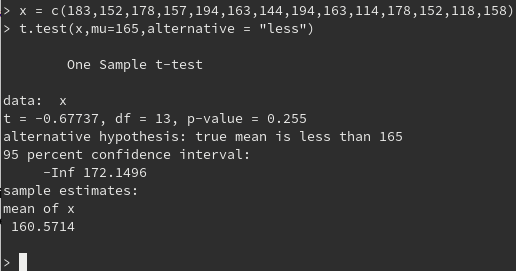
\includegraphics[width=0.8\textwidth]{prak1.png}
\end{center}
Dari output di atas diketahui t = -0,67737 dan \texttt{p-value} = 0.255
karena $p\_value = 0.255 > 0.05$ maka $H_{0}$ gagal ditolak, berarti rata-rata tekanan darah sistolik pasien lebih dari 165 mmHg.

\subsubsection{Praktik 2}
Ujilah hipotesis bahwa isi minuman kemasan X 500 ml. Bila diambil secara random 10 minuman kemasan dan diukur isinya adalah 500.2, 500. 9, 500,7,  500.1,  499.8,  499.9, 500.4,  500.3, 499.8, 500.3 ml.Gunakan taraf nyata 1\%! 

\paragraph{Jawab\\}
Dari soal di atas diketahui $\mu = 500$, jadi mu = 500. Sedangkan yang diujikan adalah kedua sisi, jadi alternative="two.sided". Dan $\alpha = 0.01$ karena yang diujikan dua sisi, maka $\alpha$\textbackslash2 jadi $\frac{\alpha}{2} = 0.005$
\begin{center}
    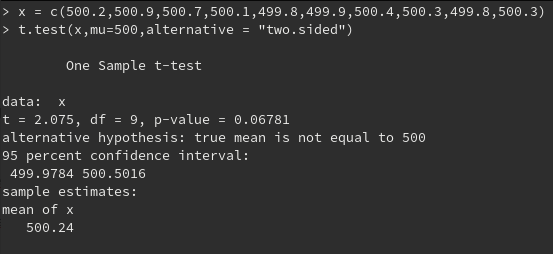
\includegraphics[width = 0.8\linewidth]{prak2.png}
\end{center}
Dari output di atas diketahui bahwa \texttt{p\_value}-nya lebih besar dari $\alpha$ ($0.06781 > 0.05$) sehingga $H_{0}$ gagal ditolak, berarti rata-rata isi minuman kemasan adalah 500ml

\newpage

\subsection{Latihan}
\subsubsection{Latihan 1}
Seorang manajer marketing  ingin mengetahui apakah web yang dibuat pada satu bulan sudah memenuhi target, yaitu minimal dikunjungi 50 pengunjung per hari. Lakukanlah uji hipotesis dengan $\alpha = 10\%$! 
\begin{table}[!ht]
    \centering
    \begin{tabular}{|l|l|l|}
        \hline
        32 & 53 & 71 \\ \hline
        35 & 64 & 69 \\ \hline
        33 & 57 & 53 \\ \hline
        38 & 66 & 55 \\ \hline
        39 & 58 & 58 \\ \hline
        37 & 67 & 63 \\ \hline
        41 & 56 & 66 \\ \hline
        45 & 66 & 62 \\ \hline
        43 & 59 & 67 \\ \hline
        47 & 63 & 70 \\ \hline
    \end{tabular}
\end{table}
\paragraph{Jawab\\}
Dari soal di atas diketahui $\mu = 50$ dan $\alpha = 0.1$, maka  perintah yang digunakan adalah\\
\texttt{t.test(x,mu=50,alternative = "less")}\\
\begin{center}
    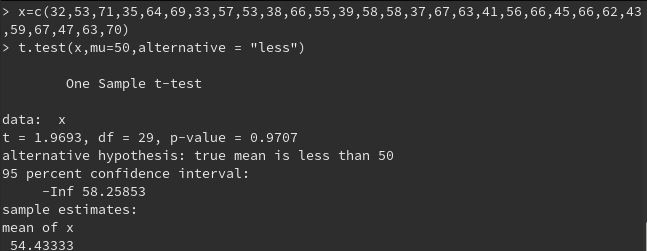
\includegraphics[width=0.8\linewidth]{lat1.png}
\end{center}
Dari output di atas diketahui \textit{p\_value} = 0.9707, karena $\alpha = 0.1$ berarti $H_{0}$ gagal ditolak, berarti jumlah pengunjung web berjumlah lebih dari sama dengan 50 pengunjung per hari.

\newpage

\subsubsection{Latihan 2}
Seorang peneliti ingin mengetahui berapakah jumlah pengunjung kantin selama 18 hari kerja sudah sesuai target pemilik kantin, yaitu 50 orang/hari. Lakukanlah uji hipotesis dengan $\alpha = 5\%$! 
\begin{table}[!ht]
    \centering
    \begin{tabular}{|l|l|}
        \hline
        35 & 53 \\ \hline
        43 & 64 \\ \hline
        51 & 42 \\ \hline
        38 & 43 \\ \hline
        60 & 58 \\ \hline
        55 & 43 \\ \hline
        50 & 36 \\ \hline
        65 & 40 \\ \hline
        38 & 58 \\ \hline
    \end{tabular}
\end{table}
\paragraph{Jawab\\}
Dari soal di atas diketahui $\mu = 50$, $\alpha = 5\%$, dan $H_{0} : \mu = \mu_{0}$, $H_{1} : \mu \neq \mu_{0}$ jadi yang diujikan adalah dua sisi(\texttt{two.sided}), jadi perintah R yang digunakan adalah:\\
\texttt{t.test(x,mu=50,alternative="two.sided")}\\
\begin{center}
    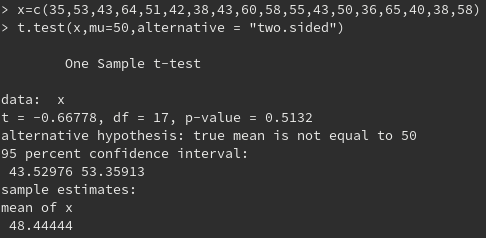
\includegraphics[width=0.8\linewidth]{lat2.png}
\end{center}
Dari output di atas diketahui bahwa \texttt{p\_value} = 0.5132, karena $\alpha = 0.05$ berarti $H_{0}$ tidak ditolak sehingga jumlah pengunjung target sudah memenuhi target.

\subsection{Tugas}
\subsubsection{Tugas 1}
Petugas parkir kampus menghitung jumlah mahasiswa yang memakai sepeda ke kampus. Pengamatan dilakukan selama 20 hari kerja. Pengamatan dilakukan untuk mengetahui apakah himbauan terhadap mahasiswa agar memakai sepeda ke kampus sudah terpenuhi, yaitu dengan melihat apakah mahasiswa yang bersepeda sudah lebih dari 40 mahasiswa/hari. Lakukanlah uji hipotesis dengan alpa = 5\%! Berikan interpretasinya! Berikut data yang diperoleh selama 20 hari :
\begin{table}[!ht]
    \centering
    \begin{tabular}{|l|l|}
        \hline
        27 & 39 \\ \hline
        33 & 32 \\ \hline
        31 & 42 \\ \hline
        38 & 43 \\ \hline
        38 & 35 \\ \hline
        40 & 34 \\ \hline
        42 & 36 \\ \hline
        36 & 40 \\ \hline
        37 & 38 \\ \hline
        41 & 43 \\ \hline
    \end{tabular}
\end{table}
\paragraph{Jawab\\}
Dari soal di atas dapat diketahui:
\begin{itemize}
    \item $\mu = 40$
    \item $\alpha = 0.05$
    \item $H_{0} : \mu \leq \mu_{0}$
    \item $H_{1} : \mu > \mu_{0}$
\end{itemize}
Sehingga perintah R yang digunakan adalah:\\
\texttt{t.test(x,mu=40,alternative="greater")}\\
\begin{center}
    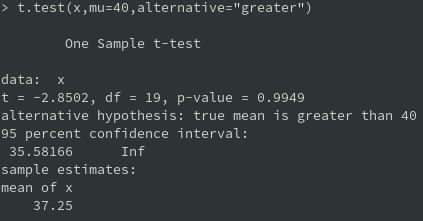
\includegraphics[width=0.8\linewidth]{tugas1.png}
\end{center}
Dari output di atas diketahui bahwa \texttt{p\_value} = 0.9949, sehingga $p\_value > \alpha$, maka $H_{0}$ tidak ditolak, berarti mahasiswa yang naik sepeda masih kurang dari 40 per-harinya

\subsubsection{Tugas 2}
Seorang peneliti ingin melakukan suatu penelitian mengenai tinggi badan mahasiswa yang mengikuti mata kuliah Statistika. Untuk itu dilakukan suatu penelitian terhadap sepuluh mahasiswa yang mengikuti mata kuliah tsb, dengan data sbb:\\
TB (cm) 185 150 156 171 160 160 165 171 166 150\\ 
Ujilah hipotesis: apakah tinggi badan mahasiswa tersebut adalah 155 cm?

\paragraph{Jawab\\}
Dari soal di atas dapat diketahui:
\begin{center}
    \item $\mu = 155$
    \item $\alpha = 0.05$
    \item $H_{0} : \mu = \mu_{0}$
    \item $H_{1} : \mu \neq \mu_{0}$
\end{center}

\end{document}
